\begin{enumerate}
\item Show that there is a perfect square that is the sum of two
perfect squares.

\hint{Can you say "Pythagorean triple"? I thought you could.}

\wbvfill

\item Show that there is a perfect cube that is the sum of three
perfect cubes.

\hint{Hint: $6^3$ can be expressed as such a sum.}

\wbvfill

\workbookpagebreak

\item Show that the \index{well-ordering principle}WOP doesn't hold in the integers.  (This is an
existence proof, you show that there is a subset of $\Integers$
that doesn't have a smallest element.)

\hint{How about even integers? Is there a smallest one?  That's my example!  You come up with a 
different one!}

\wbvfill

\item Show that the WOP doesn't hold in $\Rationals^+$.

\hint{Consider the set $\{ 1, 1/2, 1/4, 1/8, \ldots \}$.  Does it have a smallest element?}

\wbvfill

\workbookpagebreak

\item In the proof of Theorem~\ref{gcd!exists} we weaseled out of
showing that $d \divides b$.  Fill in that part of the proof.

\hint{Yeah, I'm going to keep weaseling\ldots}

\wbvfill

\item Give a proof of the unique existence of $q$ and $r$ in the
division algorithm. 

\hint{Unique existence proofs consist of two parts. First, just show existence. Then, show that if there were two of the things under consideration that they must in fact be equal.}

\wbvfill

\workbookpagebreak

\item A \index{digraph}\emph{digraph} is a drawing containing a collection of points
that are connected by arrows.  The game known as \emph{scissors-paper-rock}
can be represented by a digraph that is \emph{balanced} (each point has the
same number of arrows going out as going in).  Show that there is a 
balanced digraph having 5 points.

\begin{center}
\begin{picture}(0,0)%
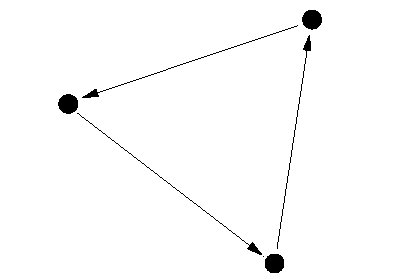
\includegraphics{./sci-pap-roc.pdf}%
\end{picture}%
\setlength{\unitlength}{3947sp}%
%
\begingroup\makeatletter\ifx\SetFigFont\undefined%
\gdef\SetFigFont#1#2#3#4#5{%
  \reset@font\fontsize{#1}{#2pt}%
  \fontfamily{#3}\fontseries{#4}\fontshape{#5}%
  \selectfont}%
\fi\endgroup%
\begin{picture}(3345,2223)(3054,-2286)
\put(5469,-1199){\makebox(0,0)[lb]{\smash{{\SetFigFont{12}{14.4}{\familydefault}{\mddefault}{\updefault}{\color[rgb]{0,0,0}smashes}%
}}}}
\put(5723,-213){\makebox(0,0)[lb]{\smash{{\SetFigFont{12}{14.4}{\familydefault}{\mddefault}{\updefault}{\color[rgb]{0,0,0}scissors}%
}}}}
\put(5381,-2271){\makebox(0,0)[lb]{\smash{{\SetFigFont{12}{14.4}{\familydefault}{\mddefault}{\updefault}{\color[rgb]{0,0,0}rock}%
}}}}
\put(3956,-1652){\makebox(0,0)[lb]{\smash{{\SetFigFont{12}{14.4}{\familydefault}{\mddefault}{\updefault}{\color[rgb]{0,0,0}covers}%
}}}}
\put(4423,-463){\makebox(0,0)[lb]{\smash{{\SetFigFont{12}{14.4}{\familydefault}{\mddefault}{\updefault}{\color[rgb]{0,0,0}cuts}%
}}}}
\put(3069,-837){\makebox(0,0)[lb]{\smash{{\SetFigFont{12}{14.4}{\familydefault}{\mddefault}{\updefault}{\color[rgb]{0,0,0}paper}%
}}}}
\end{picture}%

\end{center}
  
\hint{If at first you don't succeed\ldots \newline
try googling ``scissor paper rock lizard spock.''}

\wbvfill

\workbookpagebreak

\end{enumerate}